%%%%%%%%%%%%%%%%%%%%%%%%%%%%%%%%%%%%%%%%%%%%%%%%%%%%%%%%%%%%%%%%%%%%%%%%
% Introduction de l'étude
%%%%%%%%%%%%%%%%%%%%%%%%%%%%%%%%%%%%%%%%%%%%%%%%%%%%%%%%%%%%%%%%%%%%%%%%

\section{Présentation du cadre du stage}
%=======================================

	\subsection[LPC-Clermont]{Le Laboratoire de Physique Corpusculaire}
	%----------------------------------------------------

Le Laboratoire de Physique Corpusculaire (LPC) appartient à l'Institut de Physique Nucléaire et de Physique des Particules (IN2P3). Il s'agit d'une UMR\footnote{UMR : Unité Mixte de Recherche.} du CNRS\footnote{CNRS : Centre National de la Recherche Scientifique.} et de l'Université Blaise Pascal. Le LPC développe ses recherches dans le domaine de la physique fondamentale et des applications pluridisciplinaires grâce à une douzaine d'équipes de physique expérimentale et théorique ainsi que quatre services techniques et un service administratif.

Le LPC dispose d'un service informatique, composé de 13 personnes, et est divisé en deux parties.
	\begin{itemize}
		\item \textbf{Moyens informatiques généraux} : traitant le support technique, la maintenance, ainsi que le développement de réseaux et de fermes de calculs au LPC ;
		\item \textbf{Développement d'applications scientifiques} : traitant le développement d'applications orientées temps réel et embarqué, de calculs et de modélisations, ainsi qu'une partie développement web.
	\end{itemize}

	\begin{figure}[h]
		\centering
		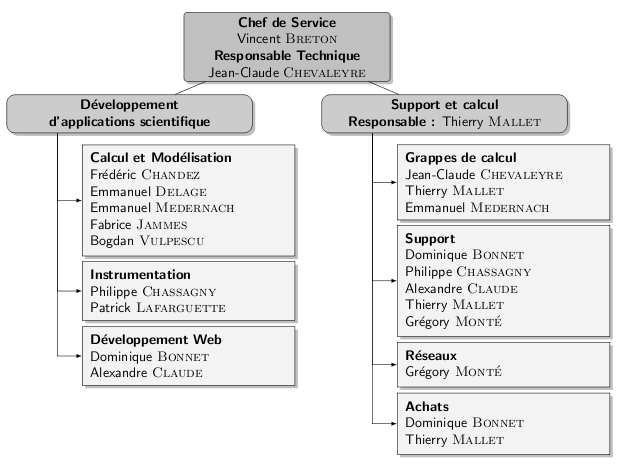
\includegraphics[width=0.65\textwidth]{img/lpc-orga-si.png}
		\caption[Organigramme du service informatique du LPC]{Organigramme du service informatique du LPC. Source : \url{http://lpc-clermont.in2p3.fr} }
	\end{figure}

J'ai eu l'occasion d'être intégré dans la partie de développement d'applications scientifiques orientées calculs et modélisations en lien avec le projet LSST.

	\begin{landscape}
		\begin{figure}[h!]
			\centering
			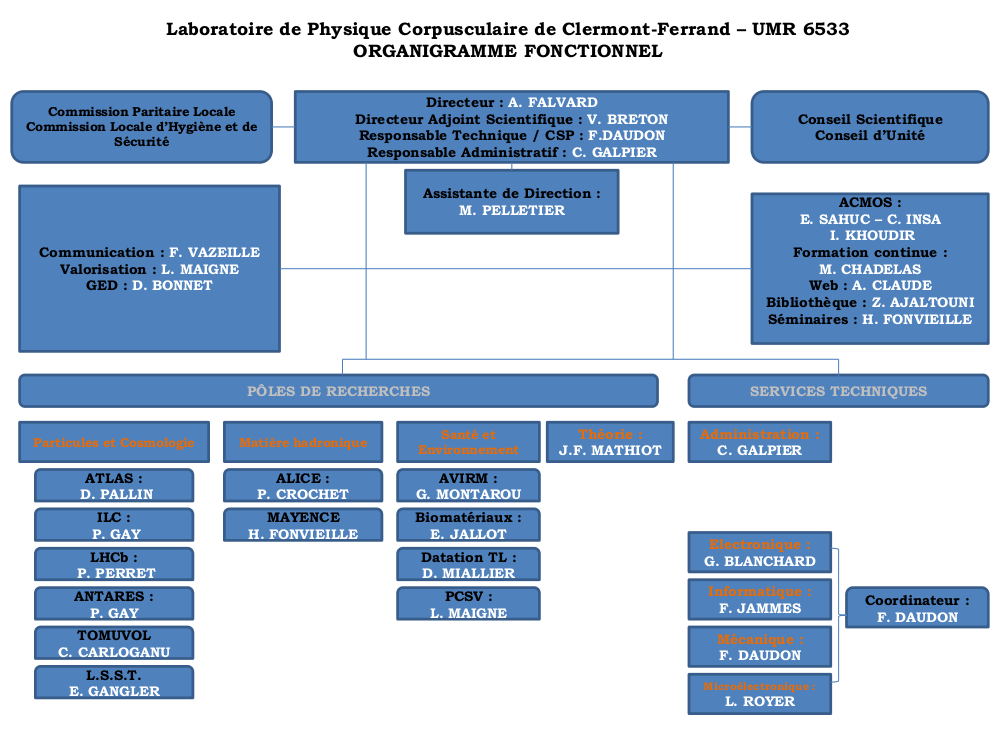
\includegraphics[height=0.95\textwidth]{img/lpc-orga.png}
			\caption[Organigramme général du LPC]{Organigramme général du LPC. Source : \url{http://lpc-clermont.in2p3.fr} }
		\end{figure}
	\end{landscape}

	\subsection{Le projet LSST}

	\begin{figure}[h!]
		\centering
		
\includegraphics[width=0.7\textwidth]{logo/Logo_LSST.png}
		\caption[Logo de LSST]{Logo de LSST.}
	\end{figure}
Le télescope LSST (\emph{Large Synoptic Survey Telescope}) est un projet mondial pour construire un télescope de surveillance continue du ciel. Il fait suite à des télescopes tels que SDSS\footnote{SDSS : télescope américain au Nouveau-Mexique de 2000 à 2007.} ou Vista\footnote{Vista : (\emph{Visible and Infrared Survey Telescope for Astronomy}) télescope de l'ESO (European Southern Observatory) au Chili à partir de 2007.} qui ont pour but de rechercher des phénomènes astronomiques brusques et non prévisibles comme les supernovæ.

Le projet LSST est piloté par le laboratoire américain SLAC (\emph{Stanford Linear Accelerator Center}). Depuis son entrée dans le consortium en 2007, la collaboration LSST France compte aujourd'hui 8 laboratoires du CNRS provenant du département de recherche IN2P3. Ces laboratoires sont, par ordre alphabétique :
	\begin{itemize}
		\item \textbf{APC} (AstroParticules et Cosmologie) (Paris), pour la calibration et le contrôle commande de la caméra et le calcul ;
		\item \textbf{\CC} (Centre de Calcul IN2P3) (Lyon), calcul et gestion des données LSST ;
		\item \textbf{CPPM} (Centre de Physique des Particules de Marseille) (Marseille), pour le changeur de filtres et le calcul ;
		\item \textbf{LAL} (Laboratoire de l'Accélérateur Linéaire) (Orsay), pour l'électronique des CCD\footnote{CCD : (\emph{Charge-Coupled Device}) il s'agit d'un capteur photométrique permettant la prise d'images astronomiques.} ;
		\item \textbf{LMA} (Laboratoire des Matériaux Avancés) (Villeurbanne), pour mener la phase d'étude de faisabilité des filtres LSST ;
		\item \textbf{LPC} (Laboratoire de Physique Corpusculaire) (Clermont-Ferrand), pour le banc de test du système d'échange de filtres , et le calcul ;
		\item \textbf{LPNHE} (Laboratoire de Physique Nucléaire et de Hautes Énergies) (Paris), pour le carrousel de filtres, le banc de caractérisation de la caméra, l'électronique des CCD et le \emph{firmware} associé à l'électronique de contrôle et de lecture des CCD .
		\item \textbf{LPSC} (Laboratoire de physique subatomique et de cosmologie) (Grenoble), pour le banc de caractérisation de la caméra et le chargeur de filtres.
	\end{itemize}

\

Trois grands sujets d'étude ressortent de cette liste, la partie \emph{caméra} ayant rapport à la construction, aux tests et au développement de l'application de contrôle de la caméra, la partie dite \emph{calcul} ayant rapport aux développements d'applications, au traitement et stockage des données ainsi que le logiciel de calibration de la caméra, et finalement une partie dite \emph{science} s'occupant de l'interprétation des résultats. Le diagramme de Gantt du projet LSST classe ces parties dans cet ordre. C'est dans la deuxième partie, \emph{calcul}, que j'ai effectué mon stage.

\section{Sujet d'étude}
%======================

	\subsection{La \emph{Data-Challange 2013}}
	%-----------------------------------------

Durant l'été 2013, un test du \stack{} sur une partie des données de SDSS a été effectué en parallèle au centre de calcul de l'IN2P3 à Lyon (CC) et aux États-Unis. Pour cela les données brutes de SDSS de la \emph{stripe 82} ont été récupérées, puis traitées par le logiciel \stack.

Pour la partie française, 300 nœuds de calculs ont été mobilisés au CC de juin à octobre, pour analyser plus de 5\,\To{} de données. Le temps total de calcul est d'environ 300\,000 heures, ce qui représente 34 ans de calculs. On voit déjà l'importance de la parallélisation des calculs qui permet d'effectuer plusieurs calculs simultanément sur plusieurs nœuds.

La base de données générées est au format MySQL, fait 4,3\,\To{} (770\,\Go{} d'index (18\%) et 3,6\,\To{} de données (82\%), c'est environ 2 milliards de lignes par table, sachant qu'il y a 5 tables. L'indexation des données prend à elle seule 15 heures de calculs par table.

		\subsubsection{Les données de SDSS}
		%^^^^^^^^^^^^^^^^^^^^^^^^^^^^^^^^^^
La \DC{} utilise une partie des données de SDSS, il s'agit de la \emph{stripe 82}, ce nom peu poétique indique la 82\up{e} région observée par SDSS, visible sur la figure~\ref{fig:sdss-skycoverage} parmi les autres régions observées par SDSS. La figure \ref{sdss:galacticequator} permet de voir la position de la \emph{stripe 82} par rapport au ciel observable, la zone bleue représentant l'équateur galactique, \ie{} la tranche visible de notre galaxie.

	\begin{figure}[h]
		\centering
		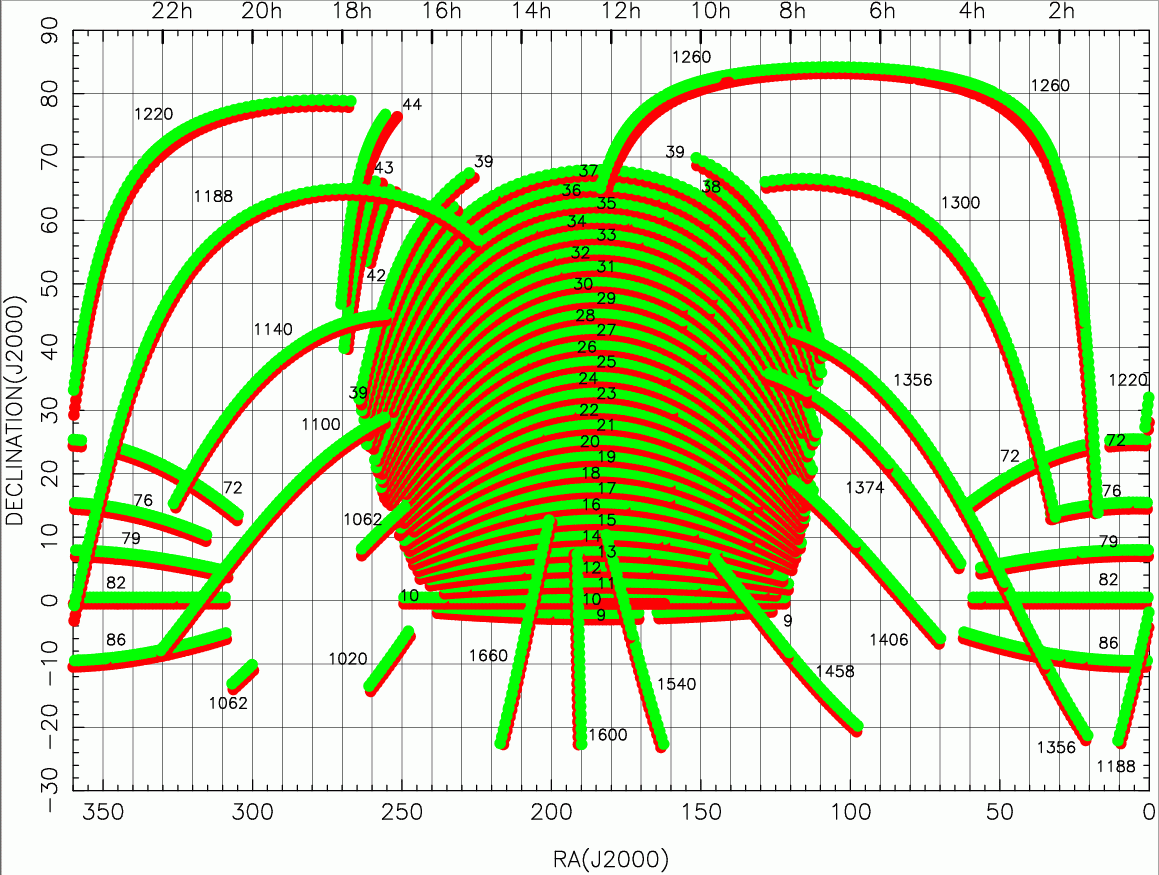
\includegraphics[width=0.8\textwidth]{img/sdss-skycoverage.png}
		\caption[Recouvrement du ciel de SDSS]{Recouvrement du ciel des images prises par SDSS ; on observe la bande 82 en bas à gauche et droite, région proche de l'équateur céleste (projection de l'équateur terrestre dans le ciel), mais éloignée de l'équateur galactique (tranche visible de notre galaxie, la Voie Lactée).}
		\label{fig:sdss-skycoverage}
	\end{figure}

	\begin{figure}[h]
		\centering
		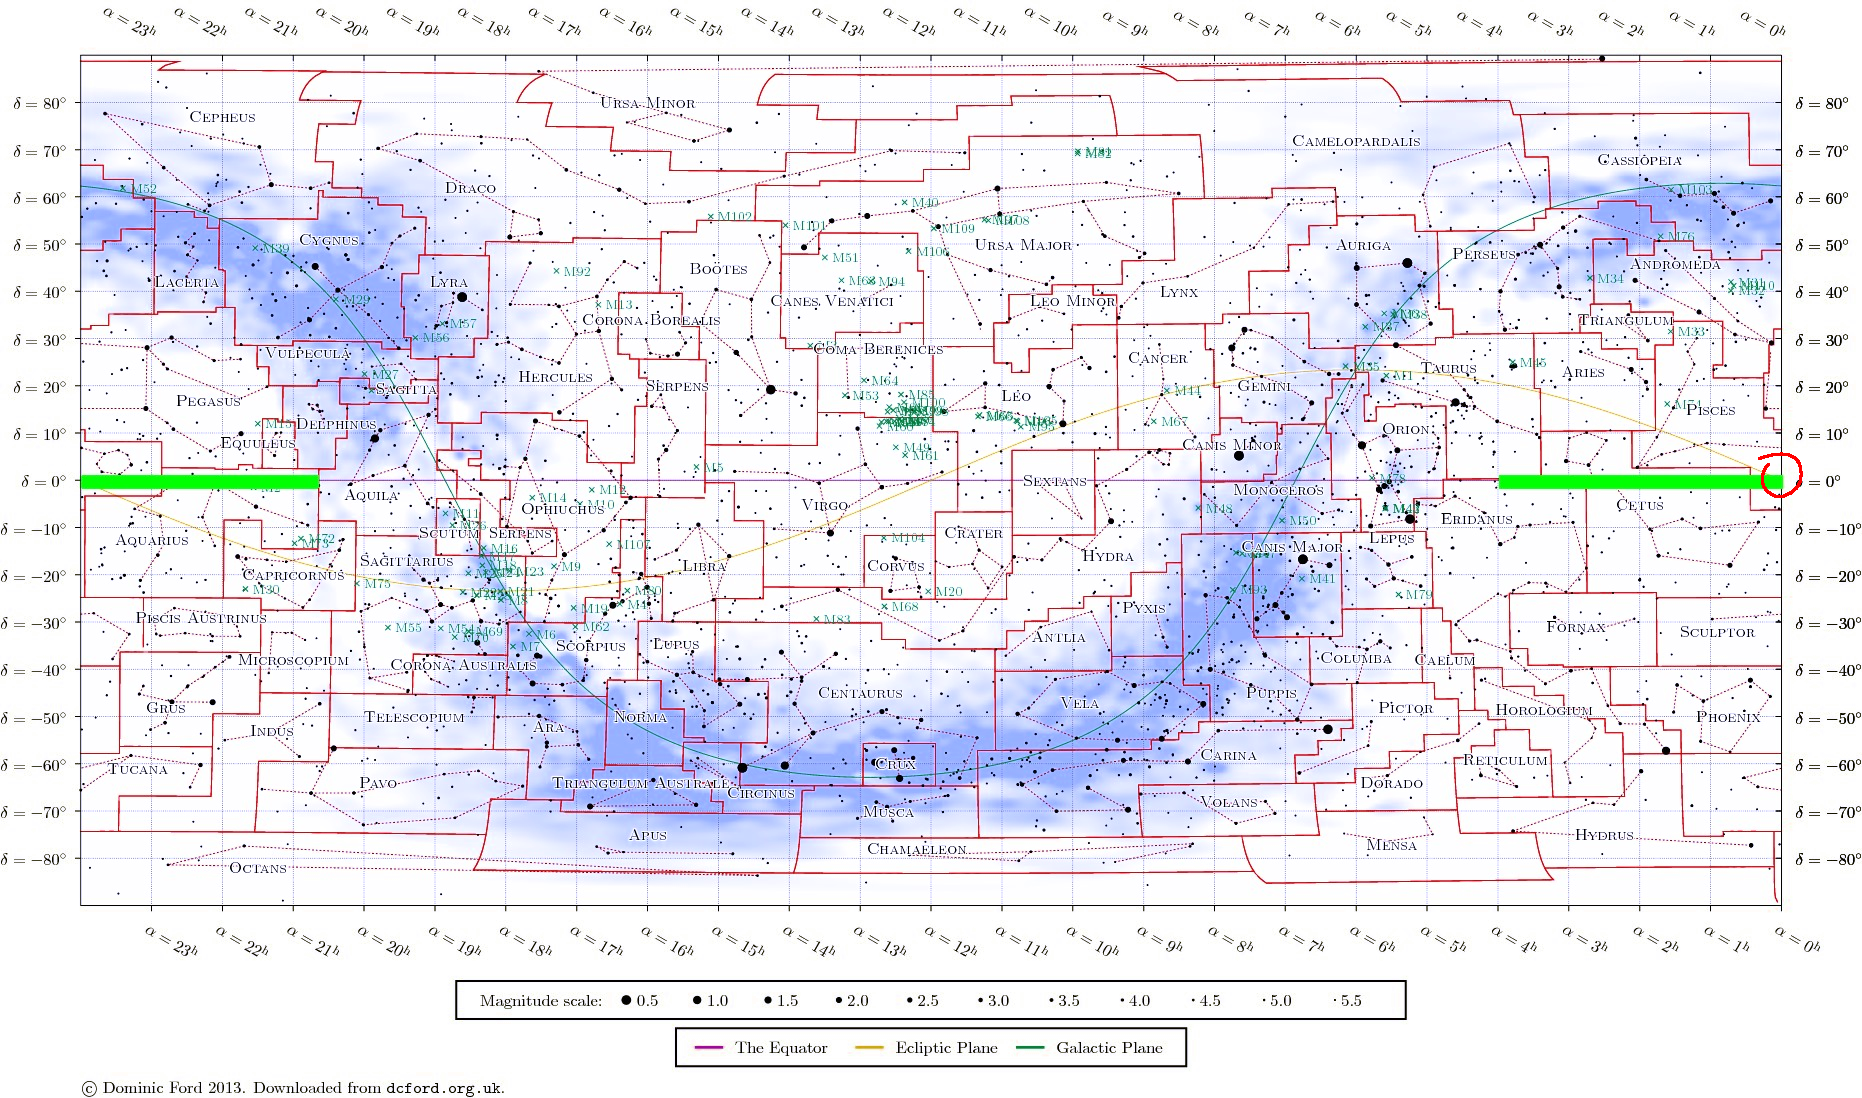
\includegraphics[width=0.8\textwidth]{img/sdss-galacticequator.png}
		\label{sdss:galacticequator}
		\caption[La \emph{stripe 82} dans le ciel]{La \emph{stripe 82} dans le ciel ; la bande 82 est la zone verte, proche de l'équateur céleste (projection de l'équateur terrestre dans le ciel), visible grâce au système de coordonnées ($0°$ en déclinaison) ; la zone bleue représente la densité d'étoiles, beaucoup plus élevée à proximité de l'équateur galactique qui est la tranche visible de notre galaxie ; la zone cerclée de rouge est approximativement la zone des $1\%$ étudiée.}
	\end{figure}

Les données de SDSS sont réparties par bandes observées, ici seule la bande 82 nous intéresse. Ces données sont subdivisées en \emph{runs}, ce qui correspond à peu près à une nuit d'observation. Ensuite le capteur de SDSS possède 5 filtres, correspondant à des longueurs d'onde différentes variant de l'ultraviolet à l'infrarouge, et 6 colonnes de capteurs. Ensuite les données sont divisées dans des fichiers \texttt{fits} correspondant à une prise de vue dans un filtre d'un des capteurs d'une colonne au moment d'une \emph{run}. Une hiérarchie analogue est disponible pour les résultats du \stack{}, les fichiers \texttt{fits} générés ne contiennent eux pas d'image, mais un tableau listant les sources identifiées par le logiciel, ainsi qu'une évaluation relative de la magnitude\footnote{La magnitude est une mesure logarithmique inverse de la luminosité, proportionnelle au flux reçu.}.

			\paragraph{Fichier \texttt{fits}}
Le format \texttt{fits} signifiant \emph{Flexible Image Transport System} est un format créé par la NASA\footnote{NASA : \emph{National Aeronautics and Space Administration}) l'agence spatiale américaine.} permettant de stocker :
	\begin{itemize}
		\item Un en-tête, contenant des données relatives à toute l'image ;
		\item Des images en une dimension (un spectre), deux dimensions, ou trois (la même image vue dans différentes longueurs d'onde) ;
		\item Une table binaire contenant une liste d'objets et des informations propres à ceux-ci.
	\end{itemize}
Plusieurs programmes et différentes API\footnote{API : (\emph{Application Programming Interface}) est une interface de programmation entre un langage de programmation et l'exécution de fonctions généralement lourdes à utiliser, cela permet de simplifier la programmation avec un niveau d'abstraction supplémentaire puisque le programmeur ne \emph{voit} pas ce qui s'effectue derrière.} permettent de lire ces fichiers et d'en extraire les données. Nous utiliserons le programme \texttt{fv} développé par la NASA pour lire les fichiers \texttt{fits}, ainsi que l'API \Python{} \texttt{pyfits} pour extraire les données dans nos programmes.

\

Pour des raisons de stockage, seuls les résultats de la \DC{} française sont accessibles à Lyon ; la différence entre les résultats des deux \DC{} ne sera pas étudiée. En réalité la différence des résultats entre la France et les États-Unis est étudiée par D\up{r} Philippe \textsc{Gris}, chercheur au LPC sur la partie des données où se situait le plus d'erreurs. Cette analyse ne faisant pas partie de l'objet de ce stage, elle ne sera qu'évoquée ici.

	\subsection{Analyse des résultats}
	%---------------------------------

Il y a différentes méthodes permettant analyser la qualité d'une base de données. La première est la comparaison avec une base de référence. Cette technique s'effectuera avec les données de SDSS. La seconde, si les données sont temporelles, consiste en l'étude de la stabilité de la base au cours du temps. Un même objet de la base peut être présent plusieurs fois mais à des instants différents compris entre 2000 et 2007 pour le cas de SDSS.

		\subsubsection{Comparaison à une autre base}
		%^^^^^^^^^^^^^^^^^^^^^^^^^^^^^^^^^^^^^^^^^^^
La comparaison à une autre base de données peut s'effectuer s'il existe déjà une base de référence dans le domaine. Dans notre cas, c'est la base de données de SDSS qui nous servira de base de référence, puisque nous avons utilisé les données brutes de SDSS. L'utilisation d'une base astrométrique tierce comme Simbad\footnote{Simbad est un catalogue de catalogues astronomiques, permettant la récupération de données d'un objet dans un catalogue particulier et de connaître les autres noms de cet objet ; en effet le nom d'un objet varie d'un catalogue à l'autre.} n'est pas exclue, mais restera au stade d'idée à cause de la difficulté de trouver un catalogue d'étoiles aussi peu lumineuses que celles observées par SDSS.

Il est fortement improbable que deux algorithmes différents de traitement d'images, celui de SDSS qui a généré la base de données SDSS et celui de LSST : le \stack, génèrent exactement le même résultat. Une comparaison exacte a l'avantage d'être très rapide, proposant de nombreux algorithmes rapides pour parcourir les deux bases de données à comparer, mais a l'inconvénient de ne pas prendre en compte le $\epsilon$ que nous rencontrerons tout au long de cette étude et que nous devons mesurer. Il est donc nécessaire de s'orienter vers une comparaison à $\epsilon$ près telle qu'une recherche de plus proche voisin. Ce domaine est riche en algorithmes, l'algorithme de base est un simple parcours des deux listes, et possède une complexité en $\mathcal{O}(n^2)$\footnote{La notation $\mathcal{O}(n^2)$ à lire « grand O de $n^2$ » signifie que dans le pire des cas, le temps d'exécution de l'algorithme est proportionnel au carré du nombre de données.}, mais l'utilisation d'arbres comme le \emph{kd-tree} permet de diminuer la complexité en $\mathcal{O}(n\log(n))$.

\

En bref, à chaque source identifiée dans la base SDSS nous essayerons d'associer une source identifiée par le \stack.

		\subsubsection{Étude de la stabilité}
		%^^^^^^^^^^^^^^^^^^^^^^^^^^^^^^^^^^^^
L'enjeu de LSST est de cartographier le ciel sur une longue période, et ainsi d'obtenir une vision temporelle d'un fond de ciel qui nous semble fixe. Il est donc intéressant de voir comment réagit l'algorithme sur la même zone du ciel mais à différents instants $t$. On peut ainsi observer la stabilité temporelle des résultats.

Le problème rencontré dans cette analyse est qu'il n'existe pas de moyen pour savoir si l'objet observé à une date $t$ est le même que celui observé à une date $t+1$. Il est donc nécessaire de trouver un moyen arbitraire pour indiquer qu'une source lumineuse à une date $t$ représente le même astre que la source observée à $t+1$.

\

L'enjeu de cette analyse est aussi d'étudier des étoiles variables, c'est à dire des étoiles dont la luminosité varie de manière importante sur des cycles relativement court (de quelques heures à 2\,000 jours). Actuellement le catalogue le plus complet sur le sujet, \emph{General Catalogue of Variable Stars}, comporte environ 40\,000 étoiles variables ou suspectées de l'être.


\section{Analyse de la tâche}
%============================

			\paragraph{Contrainte technologique}
Le travail demandé est de réaliser un programme effectuant ces analyses, comparaison à une autre base et étude de la stabilité, en utilisant le standard de programmation du projet LSST, c'est-à-dire le couple \Python/\Cpp. Ce couple est intéressant mais sera décrit plus précisément dans la deuxième partie. De plus le code développé sera majoritairement exécuté au \CC{} ; il est donc important de se contraindre à l'environnement de production.

			\paragraph{Volume des données}
La quantité des données est relativement importante. Le travail de ce stage est l'analyse de seulement 1\% des données sur le seul filtre \texttt{u}, cela représente 16\,000 paires de fichiers, pour un volume approximant les 500\,\Go. Il est donc nécessaire de réaliser un code optimisé pour le calcul, en travaillant sur la complexité, mais aussi sur la limitation des entrées-sorties.

			\paragraph{Méthode \emph{kanban}}
La méthode \emph{kanban}, signifiant « panneau » en français, est une méthode mise en place à la fin des année 50 par Toyota au Japon. Elle consiste à indiquer les tâches à faire sur un tableau divisé en 3 colonnes. La tâche arrive dans dans la première colonne, \textbf{À faire} ; lorsqu'elle est assignée, elle passe dans la colonne \textbf{En cours}, pour enfin arriver, une fois terminée et vérifiée dans la colonne \textbf{Fait}. Cette méthode permet d'observer rapidement l'état d'un projet à une date $t$. On peut y introduire un système de priorité pour faire passer des tâches urgentes plus rapidement dans la colonne \textbf{En cours}. Une représentation schématique de la méthode \emph{kanban} est visible sur la figure~\ref{fig:kanban}.

	\begin{figure}[h]
		\centering
		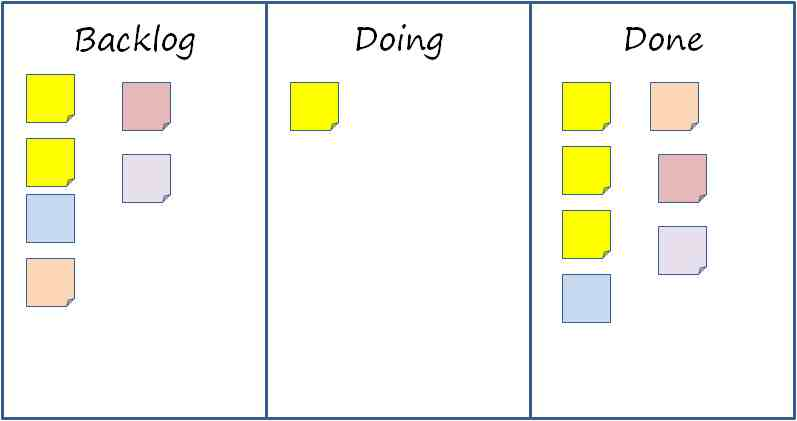
\includegraphics[width=0.7\textwidth]{img/kanban.png}
		\caption[Exemple schématique de la méthode \emph{kanban}]{Exemple schématique de la méthode \emph{kanban}, un système de couleur permet d'indiquer le groupe auquel appartient la tâche : affectation à une équipe, type de tâche, système de priorité.}
		\label{fig:kanban}
	\end{figure}

			\paragraph{Échange culturel}
Ce stage s'est déroulé dans un laboratoire de physique, la culture des physiciens et des informaticiens est différente, le vocabulaire utilisé n'est pas toujours le même, et les concepts aquis sont différents. Pour une meilleur maintenabilité du code généré au long de ce stage, j'ai pris l'initiative de privilégier la lisibilité sur l'optimisation, tout en intégrant des concepts évolués tels que la parallélisation des calculs. Une documentation complète du code ainsi que son objectif ont été réalisés. Celle-ci est à l'origine une documentation en HTML, mais une version PDF est disponible en annexe.
